\documentclass[a4paper,parskip=half,ibliography=totocnumbered,titlepage]{scrartcl}

\usepackage[T1]{fontenc}  
\usepackage[utf8]{inputenc}
\usepackage[ngerman]{babel}
\renewcaptionname{ngerman}{\figurename}{Abb.}

\usepackage{multicol}         
\usepackage{mathtools}       
\usepackage{amssymb}
\usepackage{listings}      
\usepackage{csquotes}
\usepackage{pifont}

% Tabellen
\usepackage{booktabs}
\usepackage{multirow}
\usepackage{multicol}

\usepackage{tocloft}
\renewcommand{\cftfigpresnum}{Abb. }
\settowidth{\cftfignumwidth}{Abb. 10\quad}


\usepackage{ifthen}
\newcommand{\forloop}[5][1]{%
\setcounter{#2}{#3}%
\ifthenelse{#4}{#5\addtocounter{#2}{#1}%
\forloop[#1]{#2}{\value{#2}}{#4}{#5}}%
{}}

\newcounter{crcounter}

\newcommand{\compensaterule}[1]{%
\forloop{crcounter}{1}{\value{crcounter} < #1}%
{\vspace*{-\aboverulesep}\vspace*{-\belowrulesep}}}

\newcommand{\multirowbt}[3]{\multirow{#1}{#2}%
{\compensaterule{#1}#3}}


% bibtex
\usepackage[natbib,bibencoding=auto,style=authoryear,backend=biber]{biblatex}
\bibliography{references.bib}
\DeclareLanguageMapping{ngerman}{ngerman-apa}


%Schusterjungen und Hurenkinder
\clubpenalty = 10000
\widowpenalty = 10000

%Farbnamen benutzen
\usepackage[usenames,dvipsnames]{color}

\definecolor{black}{gray}{0} % Umdefinition der Farbe black, falls noetig (0=schwarz, 1=weiss)
\definecolor{dblue}{rgb}{0.1,0.2,0.6} % Dunkelblau, fuer Hyperlinks
\definecolor{lgray}{gray}{0.9} % Hellgrau, fuer Tabellen (0=schwarz, 1=weiss)
\usepackage[hyperfootnotes=false,colorlinks=true,linkcolor=black,citecolor=dblue,urlcolor=dblue]{hyperref} 

\usepackage{setspace}

\usepackage{enumitem}
\setlist{noitemsep} % or \setlist{noitemsep} to leave space around whole list

% \begin{enumerate}[label=(\roman{*})]

\newcommand{\HRule}[1]{\rule{\linewidth}{#1}} 	% Horizontal rule

\makeatletter							% Title
\def\printtitle{%						
    {\centering \@title\par}}
\makeatother									

\makeatletter							% Author
\def\printauthor{%					
    {\centering \large \@author}}				
\makeatother							

\usepackage{lastpage}
\usepackage{fancyhdr}
\pagestyle{fancy}
\fancyhf{}
\renewcommand{\footrulewidth}{0.5pt}
\renewcommand{\headrulewidth}{0.5pt}


% ------------------------------------------------------------------------------
% Metadata (Change this)
% ------------------------------------------------------------------------------

%Kopf- und Fußzeile, jeweils links und rechts
\fancyhead[L]{Dokumentation}
\fancyhead[R]{A.R.C.S.}
\fancyhead[L]{Projekt C}
\fancyfoot[R]{Seite \thepage\ von~\pageref{LastPage}}

%Titelblat
\title{\normalsize \textsc{Dokumentation Projekt C} 	% Subtitle of the document
		 	\\[2.0cm]													% 2cm spacing
            \HRule{0.5pt} \\ [0.5cm]										% Upper rule + 0.5cm spacing
			\LARGE \textbf{\uppercase{A.R.C.S - Android Rubik's Cube Solver}}	% Title
			\HRule{0.5pt} \\ [0.5cm]								% Lower rule + 0.5cm spacing
			\large Stephan Halbritter (Matr.-Nr.: 2093970)\\
      Colin Sames (Matr.-Nr.: 2093044)\\
		}

\author{Betreuer: Prof.~Dr.~Plaß\\
    Media Systems (B.Sc.)\\
    Hochschule für Angewandte Wissenschaften Hamburg\\
}


\begin{document}
% ------------------------------------------------------------------------------
% Maketitle
% ------------------------------------------------------------------------------
\thispagestyle{empty}				% Remove page numbering on this page

\printtitle									% Print the title data as defined above
  	\vfill
\printauthor								% Print the author data as defined above
\newpage

\tableofcontents
\newpage

\section{Idee}  % sgelb 100%
Die grundlegende Idee ist simpel und mit drei Schritten erklärt:

\begin{enumerate}

  \item Nehme einen ungelösten \emph{Rubik's Cube}

  \item Lese seine Seiten über die Kamera eines Smartphones ein

  \item Folge den Anweisungen und löse den Würfel

\end{enumerate}

Hauptaugenmerk lag hierbei auf dem möglichst einfachen Einlesen der sechs
Würfelseiten mit den insgesamt 54 Farbflächen.

\section{Der Würfel}  % 100% sgelb

\begin{figure}[ht!]
  \centering
  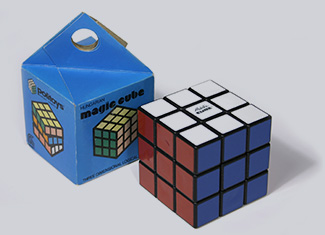
\includegraphics[width=\textwidth]{pics/rubikcube1977.jpg}
  \caption{Die ersten Exemplare wurden 1977 in Budapest verkauft
  (\cite{rubik:history})}
  \label{fig:rubik1977}
\end{figure}

Der \emph{Rubik's Cube} oder \emph{Zauberwürfel} wurde 1974 durch den
ungarischen Architekturprofessor Ernő Rubik erfunden, um seinen Studierenden
räumliche Verhältnisse anschaulicher präsentieren zu können. Seitdem beschäftigt
sich nicht nur die Mathematik immer wieder damit, der Würfel hat auch seinen
eigenen Sport, das \emph{Speedcubing} geschaffen.\footcite{rubik:history} 

\subsection{Aufbau}  % 100% sgelb

Der klassische sechsseitige Würfel aus Abbildung~\ref{fig:rubik1977} besteht aus
insgesamt 26 Teilen. Jede der sechs mittleren Flächen auf jeder Seite – die
\emph{Mittelteile} – hat eine eigene Farbe.\footnote{In der Regel sind dies
Orange, Blau, Rot, Grün, Weiß und Gelb} Sie lassen sich nicht rotieren, ihr
Position zueinander ist also festgelegt. Desweiteren gibt es zwölf
\emph{Kantensteine}, die zwei über eine Kante verbundene \emph{facelets}
verbinden und acht \emph{Ecksteine}, die drei \emph{facelets} über eine Ecke
verbinden.

\subsection{Lösungsalgorithmen}  % 100% sgelb

Insgesamt ergeben sich rund \( 4,3 \cdot {10}^{19} \) verschiedene
Kombinationen. Die maximale Anzahl von Zügen, um jeden beliebigen Würfel zu
lösen, wird \emph{God's number} genannt. Erst 2010 hat ein Team um Herbert
Kociemba durch ein Brute Force-Verfahren bewiesen, daß diese Nummer Gottes exakt
20 beträgt \citep{rubik:godsnumber}.

Zum Finden der optimalen Lösung kommt der \emph{Two-Phase}-Algorithmus zum
Einsatz. Dieser wurde erstmals von Herbert Kociemba vorgestellt
\citep{rubik:kociemba}. Wir nutzen Teile der optimierten Implementierung
von Shuang Chen, die er unter der GPLv3 auf github.com veröffentlicht
\citep{rubik:chen}.

\subsection{Notation}  % 100 % sgelb

Um die verschiedenen Züge, die es zur Lösung eines Würfels benötigt, zu
notieren, wird in der Regel auf folgendes Schema zurückgegriffen. Wenn nicht
anders angemerkt, wird sich auf eine Drehung um $90^\circ$ im Uhrzeigersinn
bezogen.

\begin{itemize}
  \item \textbf{F}ront bzw. Vorderseite
  \item \textbf{R}ight bzw. rechte Seite
  \item \textbf{B}ack bzw. Rückseite
  \item \textbf{L}eft bzw. linke Seite
  \item \textbf{D}own bzw. Unterseite
  \item \textbf{U}p bzw. Oberseite
  \item ein nachgestelltes Hochkomma \textbf{'} ändert die Rotationsrichtung gegen den
    Uhrzeigersinn
  \item eine nachgestellte \textbf{2} führt die Drehung zweimal, also um
    $180^\circ$ aus
\end{itemize}

Die Kombination \textbf{F2 B R' L} bedeutet also:
\begin{itemize}
  \item Drehe die Vorderseite um $180^\circ$
  \item Drehe die Rückseite um $90^\circ$ im Uhrzeigersinn
  \item Drehe die rechte Seite $90^\circ$ gegen den Uhrzeigersinn
  \item Drehe die linke Seite um $90^\circ$ im Uhrzeigersinn
\end{itemize}


\section{Umsetzung}  % sgelb 100%

\subsection{Bibliotheken und Tools}  % colin 0%
In diesem Kapitel werden die in diesem Projekt verwendeten Bibliotheken und
Hilfswerkzeuge vorgestellt.

\subsubsection{Java}  % 100%

Wenig überraschend wurde als Programmiersprache Java benutzt, das de facto den
Standard für die Androidprogrammierung darstellt.

\subsubsection{ADT/NDK}  % 100%

Ohne die \emph{Android Development Tools} und ihrer Vielzahl an in Eclipse
integrierten Tools wäre die Entwicklung nicht denkbar gewesen. Der Einsatz des
\emph{Native Development Kit} war notwendig, da das OpenCV SDK auf
C++-Bibliotheken aufbaut, über die so zugegriffen werden konnte.

\subsubsection{OpenCV}  % 100%

OpenCV ist eine in C und C++ geschriebene Bibliothek. Sie stellt eine große
Fülle an Funktionen zur Bildmanipulation und -erkennung zur Laufzeit zur
Verfügung. Mittels der \emph{OpenCV for Android
SDK}\footnote{\url{opencv.org/platforms/android.html}} wurden hiermit die Farben
der einzelnen Würfelflächen erkannt. Zum Einsatz kam OpenCV in der Version 2.4.9.

\subsubsection{Eclipse}  % 100%

Zur Programmierung haben wir auf Eclipse zurückgegriffen. Dafür sprachen mehrere
Gründe: zum damaligen Zeitpunkt war Eclipse die Standard-IDE zur
Androidentwicklung\footnote{Zumindestens nach Wünschen von Google soll diese
Rolle in Zukunft von \emph{Android Studio} eingenommen werden.}, das OpenCV SDK
war hierfür entwickelt worden und zu guter Letzt waren wir beide damit vertraut.

Eclipse bietet zudem die Möglichkeit, sehr einfach Tests mittels JUnit zu
schreiben. Tests sind sehr wichtig für dieses Projekt gewesen und haben mehrere
Male Fehler entdeckt, die leicht zu übersehen, auf längere Frist aber
schwerwiegend gewesen wären.

\subsubsection{Git}  % 100%

Als Versionsverwaltungssoftware haben wir Git gewählt, zur gemeinsamen
Codeverwaltung griffen wir auf GitHub zurück.

GitHub bietet zudem den Vorteil, dass es diverse Werkzeuge zur Projektplanung zur
Verfügung stellt. So ist es möglich, in einem Webinterface Milestones zu
definieren, Issues anzulegen und Aufgaben zuzuordnen. Das vereinfacht die
Planung ungemein.

Unsere Branching-Struktur folgt in einer vereinfachten Form dem Vorschlag von
Vincent Driessen \citep{git:driessen}: es gibt einen master-Branch, von dem aus
für vorher festgelegte Aufgaben (in Github \emph{Issues} genannt) ein Branch
erstellt wird. Ist die Aufgabe umgesetzt, wird der Branch wieder in den master
zurück gemergt. So bleiben die einzelnen Arbeiten voneinander getrennt, es gibt
mit master einen immer stabilen Zweig und das parallele Arbeiten gelingt zumeist
ohne Probleme.

Wir haben bewusst auf das EGit Plugin für Eclipse verzichtet. Stattdessen haben
wir auf das \emph{Ur-Git}, dem Kommandozeilenprogram, zurückgegriffen. Da beide
Projektmitglieder Linux zur Entwicklung nutzen, stellte das kein Problem dar.

\begin{figure}[ht!]
  \centering
  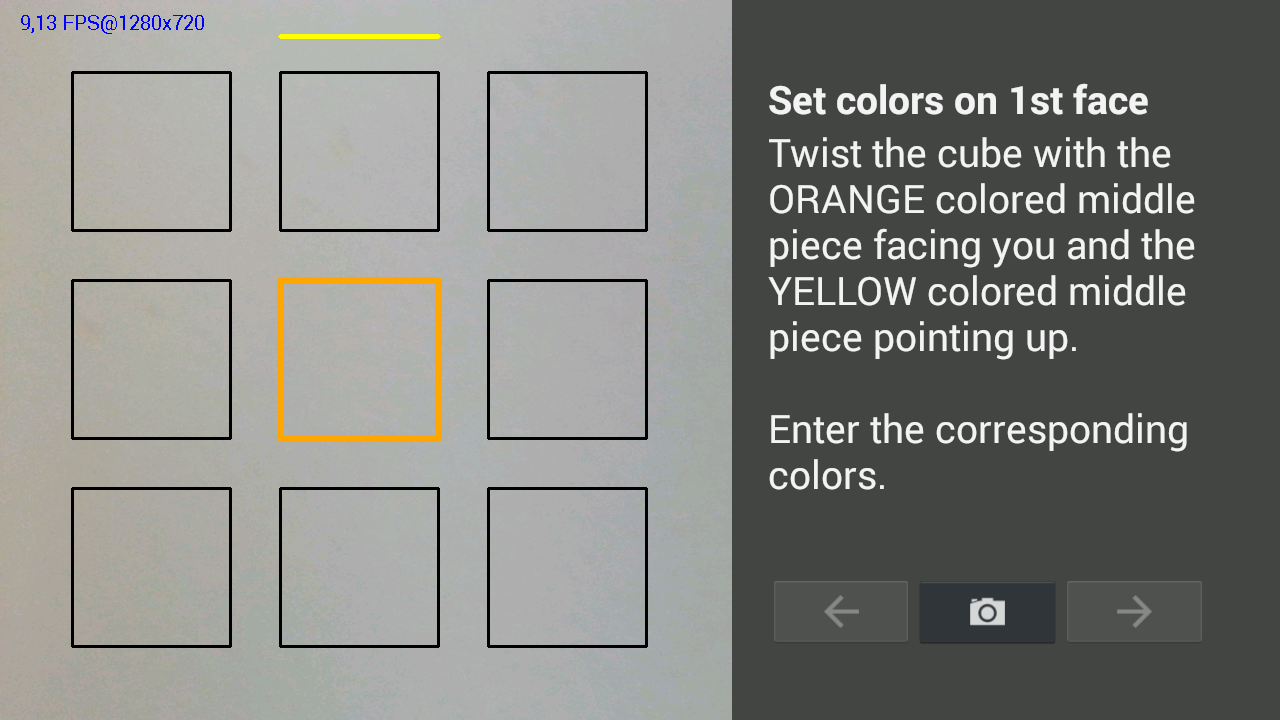
\includegraphics[width=\textwidth]{pics/arcs_unsolved.png}
  \caption{Das graphische Interface zum Einlesen der Würfelseiten.
  (Selbst erstellter Screenshot)}
  \label{fig:arcs_unsolved}
\end{figure}


\subsection{Gestaltung}  % sgelb 100%

Auch wenn die Gestaltung des Programmes nicht im Vordergrund stand, sollte die
Bedienung unkompliziert und nach Möglichkeit selbsterklärend sein. Es gibt zwei
Hauptansichten: eine für das Einlesen eines Würfels, eine für das Präsentieren
der Lösungsschritte (siehe Abbildung~\ref{fig:arcs_solving}). Der grundlegende
Aufbau der Oberfläche ist bei beiden der gleiche. Die Anzeige erfolgt im
Querformat. Auf der linken Seite wird eine Würfelseite angezeigt. Auf der
rechten Seite gibt konkrete Anweisungen für den User. Unter den Anweisungen
sind, leicht mit dem Daumen der rechten Hand zu bedienen, die notwendigen
Buttons angezeigt. Für die Darstellung wurde wenn möglich auf Standardelemente
der Android-API zurückgegriffen, das Einblenden der Kameransicht wurde über die
OpenCV-API realisiert.

\subsection{Arbeitsprozess}  % sgelb 100%

Am Anfang stand die Planung der zu erreichenden Ziele. Wir haben vier Milestones definiert:

\begin{enumerate}
  \item Implementierung des Code-Grundgerüstes, also der Klassen für den Würfel,
    die Rotation u.ä.
  \item manuelle und automatisierte Eingabemöglichkeiten für den Würfel
  \item Berechnung der Lösung
  \item Anzeigen der Lösung
\end{enumerate}

\begin{figure}[ht!]
  \centering
  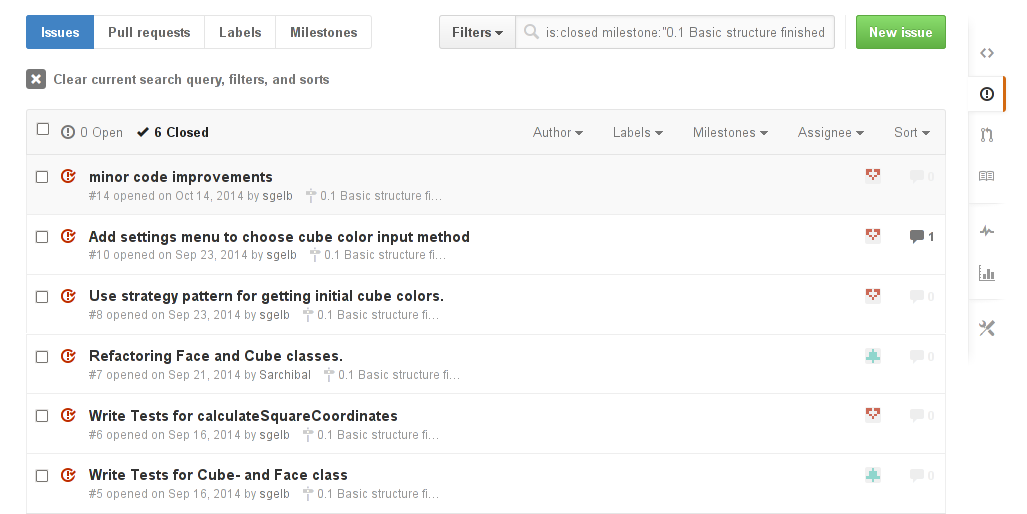
\includegraphics[width=\textwidth]{pics/github_issues.png}
  \caption{Die sechs Issues des ersten Milestones in der Github-Ansicht.
  (Selbst erstellter Screenshot)}
  \label{fig:github_issues}
\end{figure}

Jeder Milestone setzte sich aus mehreren Issues zusammen.
Abbildung~\ref{fig:github_issues} zeigt die Issues für den ersten Milestone und
wer sich für das Lösen verantwortlich zeigt.

Aus unseren Erfahrungen mit den vorherigen Projekten beschlossen wir, uns
regelmässig einmal die Woche zu treffen. Diese Treffen erfüllten mehrere Ziele:
in einer Nachbetrachtungsphase berichteten und zeigten wir einander, an was wir
seit dem letzten Treffen gearbeitet hatten und versuchten, uns auf den gleichen
Stand in Bezug auf die Kenntnis des Codes zu bringen. In der Planungsphase
überlegten wir uns Lösungsansätze für eventuell aufgetretende Probleme und
welche Issues wir als nächstes angehen sollten. Am Ende stand oftmals das
Vereinbaren eines Termines zum gemeinsamen Programmierens.


\section{Benutzung}  % colin 0%

Die Android-App \emph{A.R.C.S.} ist eine App zur Lösung eines Rubiks Cube.
Nach dem Starten der App bekommt der User eine GUI im Querformat zu sehen.

Die linke Hälfte nimmt das Kamerafeld ein, rechts sind eine Beschreibung sowie
drei Buttons zu sehen. Auf dem Kamerafeld links befinden sich, den Farbfeldern

Möchte der User den Würfel halbautomatisch einlesen, so hält er den Würfel in
der richtigen Ausrichtung in die Kamera. Die korrekte Position lässt sich
mittels der vorkonfigurierten Farbe des mittleren Feldes und des Farbbalken am
oberen Rand bestimmen. Der Farbbalken zeigt die Farbe (des mittleren
Feldes) der oberen Seite an und ermöglicht so eine eindeutige Ausrichtung der
Seiten.

Der User hält nun die richtige Seite in die Kamera und achtet darauf, dass sich
jedes Feld auf dem Würfel in einem Quadrat auf dem Bildschirm befindet. Hat der
User den Würfel richtig positioniert, so kann er auf den Button mit Kamerasymbol
klicken. Es wird nun versucht, die korrekten Farben zu erkennen. 

\begin{figure}[ht!]
  \centering
  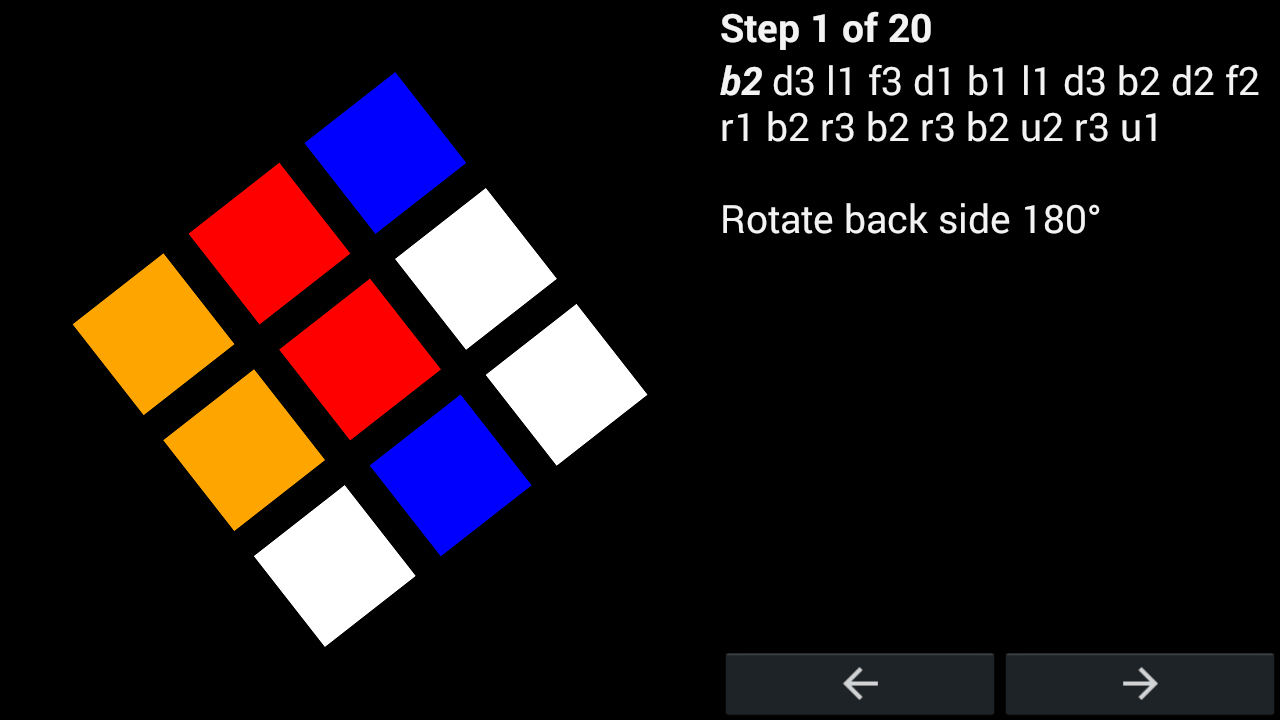
\includegraphics[width=\textwidth]{pics/arcs_solving.png}
  \caption{Ansicht des ersten Lösungsschrittes. Die Würfelansicht ist animiert.
  (Selbst erstellter Screenshot)}
  \label{fig:arcs_solving}
\end{figure}

Es ist auch möglich, jedes Feld manuell zu setzen. Ein Touch auf ein Feld öffnet
ein Auswahlmenü mit den sechs Farben.\footnote{Ein Touch auf das mittlere, bereits
definierte Feld färbt die gesamte Seite einfarbig ein und diente vor allem dem
Debugging.} So lassen sich leicht falsch erkannte Felder korrigieren.

Zusätzlich bietet das \emph{Settings}-Menü die Möglichkeiten, alle bereits
gesetzten Farbwerte zu löschen oder mit Farben eines lösbaren, aber zufälligen
Würfels zu füllen.

Erst wenn alle neun Felder eine Farbe zugeteilt bekommen haben, wird der
"Weiter"-Button freigeschalten und der User kann die nächste Seite einlesen.
Selbstverständlich werden dabei die farblichen und textlichen Hinweise
angepasst. Es ist jederzeit möglich, zu bereits definierten Seiten
zurückzukehren. Sind alle Farben auf allen Seiten gesetzt, ist der
"Lösen"-Button freigeschalten. Sollte es ein Problem mit dem eingelesenen Würfel
geben, gibt es darauf einen Hinweis und der User erhält die Möglichkeit, das
Problem zu lösen. Andernfalls berechnet die App die Lösung und wechselt in den
Lösungsmodus.

Im Lösungsmodus (Abbildung\ref{fig:arcs_solving}) sieht der User auf der linken
Seite eine Ansicht der zu drehenden Seite. Die notwendige Rotation wird durch
eine Animation dargestellt. Zusätzlich wird auf der rechten Seite eine Übersicht
über alle notwendigen Schritte angezeigt, in welchem Schritt er sich befindet
und was er konkret tun muss. Jeder Schritt kann mit Navigationsbuttons
nacheinander aufgerufen werden. Nachdem der User alle Schritte befolgt hat,
sollte der Rubiks Cube gelöst sein.

\section{Architektur}  % colin 0%

\subsection{Hierarchie}  % 0%

Das Projekt lässt sich in vier logische Bereiche unterteilen, die in eigenen
\emph{packages} zusammengefasst sind:

\begin{itemize}
  \item der \emph{Würfel} (\texttt{com.github.sgelb.arcs.cube})
  \item die \emph{Eingabe} (\texttt{com.github.sgelb.arcs.input})
  \item der \emph{Lösungsalgorithmus} (\texttt{cs.min2phase})
  \item der \emph{Lösungsweg} (\texttt{com.github.sgelb.arcs.solution})
\end{itemize}

Die Klassen in \texttt{arcs.cube} sind für die (interne) Darstellung des Würfels
und der auf ihn anwendbaren Operationen wie der diversen Rotationsmöglichkeiten
zuständig.

Im Paket \texttt{arcs.input} ist eine Klasse für das Einlesen des Würfels
definiert. Der Zugriff läuft, entsprechend dem Strategiemuster, über eine
\emph{Interface}-Klasse. So ist sichergestellt, dass das Implementieren
zusätzlicher Einlesemöglichkeiten relativ unkompliziert möglich ist.

Für das Finden der optimalen Lösung nutzen wir die in \texttt{cs.min2phase}
enthaltenen Klassen.

\texttt{arcs.solution} enthält alles, um die Lösung schrittweise zu
präsentieren.

\subsection{Activites}

Aus der Perspektive des Users betrachtet besteht das Projekt aus vier
verschiedene Ansichten und somit auch vier verschiedene \emph{Activities}:

\begin{itemize}
  \item MainActivity
  \item SolutionActivity
  \item SettingsActivity
  \item AboutActivity
\end{itemize}

Wie in \emph{Android}-Projekten üblich, ist \texttt{MainActivity} in
\texttt{AndroidManifest.xml} als \emph{Launcher} definiert und stellt somit den
Einstieg in das Programm dar.

Die Hauptfunktion der \texttt{MainActivity} ist neben der Initialisierung der
App das Einlesen der Würfelseiten.

Hierfür stellt sie die graphische Oberfläche dar, wie sie in
Abbildung~\ref{fig:arcs_unsolved} zu sehen ist und ermöglicht darüber die
Interaktion mit dem User.

Um das Bild der Kamera in Echtzeit darzustellen, erbt \texttt{MainActivity} von
der \emph{OpenCV}-Klasse \texttt{CvCameraViewListener2}. Da der Kamerainput auch
zur automatische Erkennung der Farben notwendig ist, wird jeder Frame an eine
Instanz von \texttt{FaceInputMethod} weitergegeben.

Zur Verwaltung der aktuellen Würfeldefinition dient ein Objekt vom Typ
\texttt{RubiksCube}.

Die Anweisungstexte werden über diverse \emph{Views} angezeigt. Die drei Buttons
sind über \emph{EventListener} mit entsprechenden Funktionen verbunden. Im Falle
der \emph{Next}- und \emph{Previous}-Buttons wird getestet, ob eine vorherige
oder nächste Seite angezeigt werden kann und gegebenfalls die Ansicht geändert.
Ist der gesamte Würfel eingegeben, ruft der \emph{Solve}-Button die innere
Klasse \texttt{CubeSolver} auf. Diese übergibt die Würfeldefiniton an
\texttt{Search.soltuion()}. Damit das Userinterface nicht blockiert wird, erbt
\texttt{CubeSolver} von \texttt{AsyncTask}, läuft also in einem eigenen Thread.

Ist eine Lösung gefunden, wird diese über \texttt{Intent.putExtra()} an
\texttt{SolutionActivity} weitergegeben, welche dann gestartet wird. Hier wird
der Lösungsweg in seine einzelnen Schritte unterteilt und der Text und Animation
angezeigt.


% Bis hierher fertig

\begin{figure}[ht!]
  \centering
  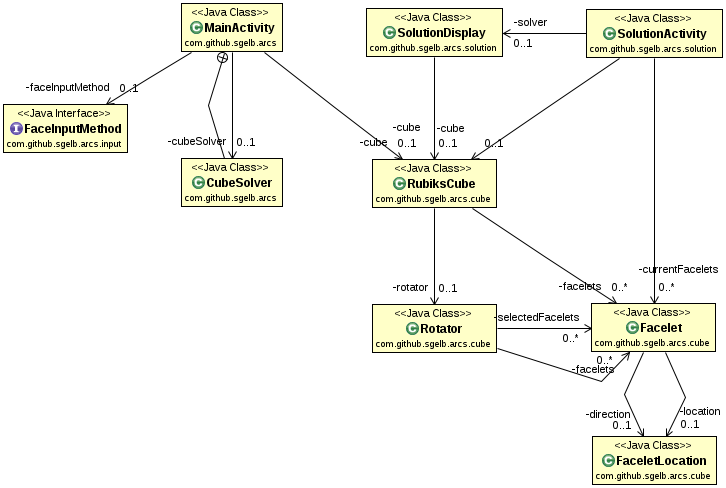
\includegraphics[width=\textwidth]{pics/uml.png}
  \caption{UML-Diagram (selbst erstellt)}
  \label{fig:uml}
\end{figure}


\subsection{Würfel}

Der Würfel an sich besteht aus mehreren Komponenten, dem Rotator, dem
CubeUpdator und den Facelets, alles eigene Klassen. Bei den Facelets handelt es
sich um ein Array der größe 54. 54 deshalb, weil dass die Anzahl der Felder ist,
die ein Rubiks Cube hat. Jedes dieser Facelets ist eine eigene Instanz des
Facelet Objekts.

\subsubsection{Facelets}

Facelets sind die Elementarsten bestandteile des Würfels. Sie enthalten die
Position des Feldes, die Richtung, in die sie zeigt und ihre Farbe. Position und
Ausrichtung sind wieder eigene Objekte, die einfache Integerwerte zu dieser
Bestimmung enthalten.

\subsubsection{Rotator}

Der Rotator, der mit den Facelets arbeitet, besitzt die Funktionen, diese
Facelets zu drehen. Aufgrund der mathematischen Eigenschaften der Facelets ist
es möglich anhand ihrer Position einfache Drehungen im Raub auszuführen, wenn
man diese Position als einen Vektor vom Uhrsprung aus betrachtet, der im Zentrum
des Würfels liegt.

\subsubsection{CubeUpdater}

Der CubeUpdater hat die Aufgabe, die in dem Rotator gedrehten Facelets auf dem
RubiksCube zu übertragen. RubiksCube und Rotator haben somit ihre eigenen
Facelets, welche durch diese Klasse synchron gehalten werden.

All diese Objekte, in stark vereinfachtet Darstellung, bilden das Grundgerüst
für diese App.

\subsection{Input}

Die Usereingabe wird duch die Input Klassen bereitgestellt. Sie berechnen auch
die Farben des automatische Einlesen über die Kamera. Auch sie werden in der
MainActivity instanziiert.

\subsection{Solution}

BLABLA




\subsection{Prinzipien}  % 0%
Alle Prinzipien, namentlich Single Responsibility Principle (SRP), Open Closed
Principle (OCP) und Dont Repeat Yourself (DRP), wurden nach besten Gewissen stets
eingehalten und ziehen sich durch dieses Projekt.

\section{Auswertung und Fazit}  % sgelb 0%

Das Projekt ist zu unserer Zufriedenheit verlaufen und wir konnten alle
festgelegten Ziele und Features umsetzen. Wir haben viel gelernt was App
Entwicklung angeht, mit allen seinen Facetten, z.B. Design und Layout, aber auch
das Programmieren hat uns vor Aufgaben gestellt, die uns forderten und
förderten, und der Mensch wächst schließlich mit seinen Aufgaben und
Herausforderungen. Die Zusammenarbeit funktionierte einwandfrei und war stets
motivierend, was die Voraussetzung eines erfolgreichen Projektes bildet. Das
wichtigste jedoch ist die Aussage, dass wir zufrieden mit dem Erreichten sind
und wir sind zufrieden.


% Am Ende Bild- und Quellenverzeichnis
\appendix
\printbibliography[heading=bibintoc,title={Quellenverzeichnis}]
\listoffigures

\end{document}
